\section{问题三：逐点达标判据下的烘干时长确定}

\subsection{相对问题二的改动：达标判据的数学定义}

本问的模型与问题二完全相同：同样的式~\eqref{eq:energy}--\eqref{eq:ic}、
同样的式~\eqref{eq:prop_app3} 物性、同样的固定域 $R=2$~cm。唯一新增的是一个终止条件。
新增内容虽只有一式，但它的定义方式直接决定答案，因此需要单独论证。

干燥过程中含水率沿半径始终不均匀。由表~\ref{tab:p2_C} 可见同一时刻中心最高、表面最低，
两者可相差数倍。要保证「药材内部含水率降到 $0.15$~kg/kg 以下」，
必须要求最难干的位置也达标，故把达标时刻定义为逐点最大含水率首次低于阈值的时刻

\begin{equation}\label{eq:tend}
t_{\rm end}=\min\Bigl\{\,t>0 \;\Bigm|\; \max_{0\le r\le R} C(r,t) < C_{\rm th}\,\Bigr\},
\qquad C_{\rm th}=0.15~\mathrm{kg/kg}.
\end{equation}

与式~\eqref{eq:tend} 相对的是以体平均含水率判定的做法

\begin{equation}\label{eq:cbar}
\bar C(t)=\frac{\displaystyle\int_0^R C(r,t)\,2\pi r\,\mathrm{d}r}{\pi R^2},
\end{equation}

式~\eqref{eq:cbar} 把径向分布压成一个数，必然在芯部尚未达标时就先跨过阈值，
从而给出偏短的时长。本文只把 $\bar C$ 作为对照量输出，不用作判据。
由式~\eqref{eq:bc_center} 的对称条件与解的单调性，含水率最大值总出现在轴心，
故式~\eqref{eq:tend} 的控制点即 $r=0$。

数值实现上，$C_{\max}(t)$ 只在离散输出步上可得，而阈值一般落在两个输出步之间。
为不使时长精度受输出间隔限制，在跨越阈值的相邻两步之间对 $C_{\max}$ 作线性插值

\begin{equation}\label{eq:interp}
t_{\rm end}\approx t^{n}+\Delta t\,
\frac{C_{\max}(t^{n})-C_{\rm th}}{C_{\max}(t^{n})-C_{\max}(t^{n+1})},
\end{equation}

式~\eqref{eq:interp} 要求 $C_{\max}(t^n)\ge C_{\rm th}>C_{\max}(t^{n+1})$，
即定位的是首次跨越而非任意一次低于阈值的时刻。

\subsection{烘干时长与含水率分布}

以 $\Delta t=1$~s 推进求解，得到烘干时长

\begin{equation}\label{eq:p3_answer}
t_{\rm end}=56.706~\mathrm{h}\approx 2.36~\mathrm{d},
\end{equation}

该时刻的逐点最大含水率为 $0.150000$~kg/kg，恰好落在阈值上，控制点位于轴心。
式~\eqref{eq:p3_answer} 与题目所述「烘干过程一般持续 2--3 天」的量级一致。
各时刻的含水率分布见表~\ref{tab:p3_C}。

\begin{table}[H]
\centering
\caption{烘干过程中药材内部水分浓度（kg/kg）}\label{tab:p3_C}
\begin{tabular}{cccccc}
\toprule
时间 (h) $\backslash$ 距中心距离 (cm) & 0 & 0.5 & 1 & 1.5 & 2 \\
\midrule
6  & 1.0156 & 0.9869 & 0.9006 & 0.7546 & 0.5334 \\
12 & 0.4548 & 0.4419 & 0.4020 & 0.3290 & 0.1641 \\
18 & 0.2979 & 0.2906 & 0.2678 & 0.2244 & 0.0847 \\
24 & 0.2369 & 0.2318 & 0.2158 & 0.1844 & 0.0665 \\
30 & 0.2049 & 0.2009 & 0.1882 & 0.1628 & 0.0597 \\
36 & 0.1850 & 0.1816 & 0.1708 & 0.1491 & 0.0565 \\
42 & 0.1712 & 0.1682 & 0.1587 & 0.1395 & 0.0547 \\
48 & 0.1610 & 0.1583 & 0.1497 & 0.1323 & 0.0535 \\
54 & 0.1530 & 0.1506 & 0.1427 & 0.1266 & 0.0528 \\
烘干结束时间 56.706 h & 0.1500 & 0.1476 & 0.1400 & 0.1244 & 0.0525 \\
\bottomrule
\end{tabular}
\end{table}

表中每一行都保持中心含水率最高、表面最低的次序，与式~\eqref{eq:tend} 取轴心为控制点相符。
前 $12$~h 中心含水率由 $2.55$ 降至 $0.4548$~kg/kg，减少了八成；而从 $12$~h 到 $56.706$~h
的四十余小时只再减少 $0.30$~kg/kg。也就是说约五分之四的水分在前四分之一的时间内被除去，
剩下的时间几乎全部花在把中心含水率从 $0.45$ 压到 $0.15$~kg/kg 上。
末行还显示表面含水率已降至 $0.0525$~kg/kg，远低于阈值，中心与表面相差近三倍——
这正是不能用平均量判定的直接证据。

判据本身的差别有多大，可由同一次求解的两条曲线读出，见图~\ref{fig:q3_drying_curve}。

\begin{figure}[H]
  \centering
  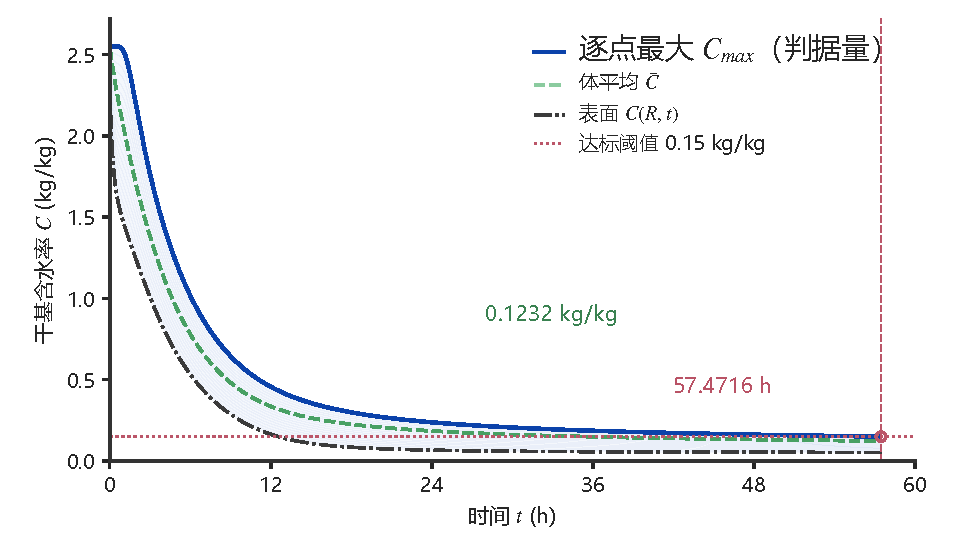
\includegraphics[width=0.9\textwidth,height=0.8\textheight,keepaspectratio]{../figures/fig_q3_drying_curve.pdf}
  \caption{问题三干燥曲线与达标时刻定位}
  \label{fig:q3_drying_curve}
\end{figure}

图中渐变带表示同一时刻药材内部由表面到芯部的含水率分布范围，带宽即内部不均匀度。
$C_{\max}$ 触及阈值时体平均含水率只有 $0.1232$~kg/kg，已低于阈值约 $18\%$；
若改用式~\eqref{eq:cbar} 判定，会在芯部含水率尚有 $0.18$~kg/kg 左右时
就宣布干燥完成。图中标注的时刻取自效应隔离基线情景（时间步长较粗），
为 $56.709$~h，与式~\eqref{eq:p3_answer} 的交付值相差 $0.003$~h，
即 $0.005\%$——两个不同时间步长下的达标时刻一致到三位有效数字，
这本身也构成时间步无关性的一项旁证。

剖面形态随时间的演化见图~\ref{fig:q3_ridgeline}。

\begin{figure}[H]
  \centering
  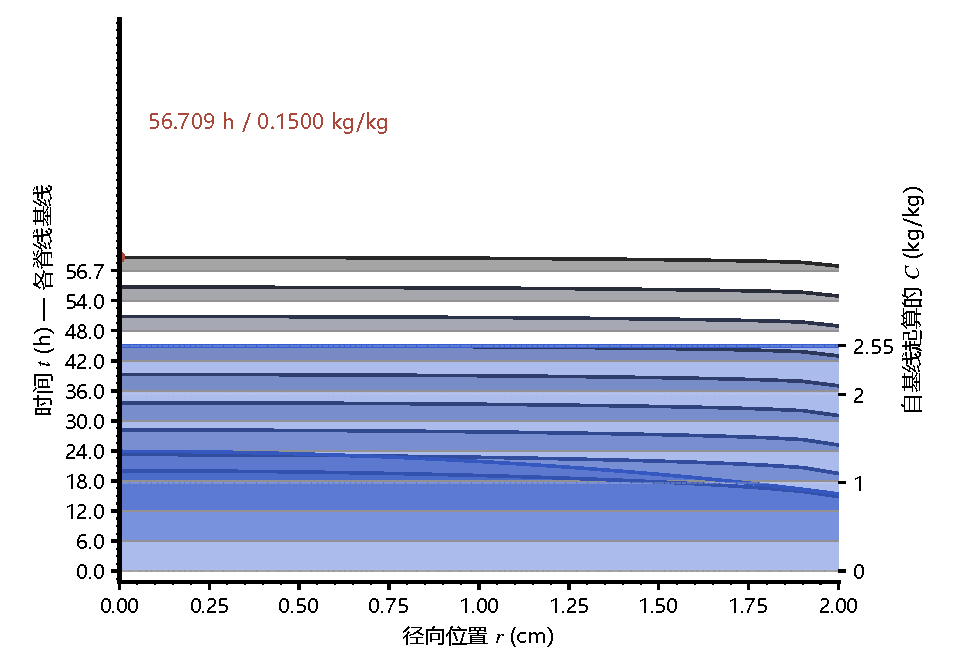
\includegraphics[width=0.9\textwidth,height=0.8\textheight,keepaspectratio]{../figures/fig_q3_ridgeline.pdf}
  \caption{问题三含水率剖面的时序脊线}
  \label{fig:q3_ridgeline}
\end{figure}

各条脊线按 $6$~h 取样、基线逐条下移。剖面形态由初期的近平坦逐步转为中心高、表面低的
抛物型，末条脊线的峰值 $0.1500$~kg/kg 即式~\eqref{eq:tend} 的临界状态。
脊线间距在后期明显收窄，与表~\ref{tab:p3_C} 中后四十小时降幅有限的读数一致。

\subsection{干燥速率的阶段特征}

干燥文献常把过程分为升速段、恒速段与降速段，其中恒速段由表面蒸发控制、
降速段由内部扩散控制。本题属于哪一类需要用实际速率曲线回答，见图~\ref{fig:q3_rate_curve}。

\begin{figure}[H]
  \centering
  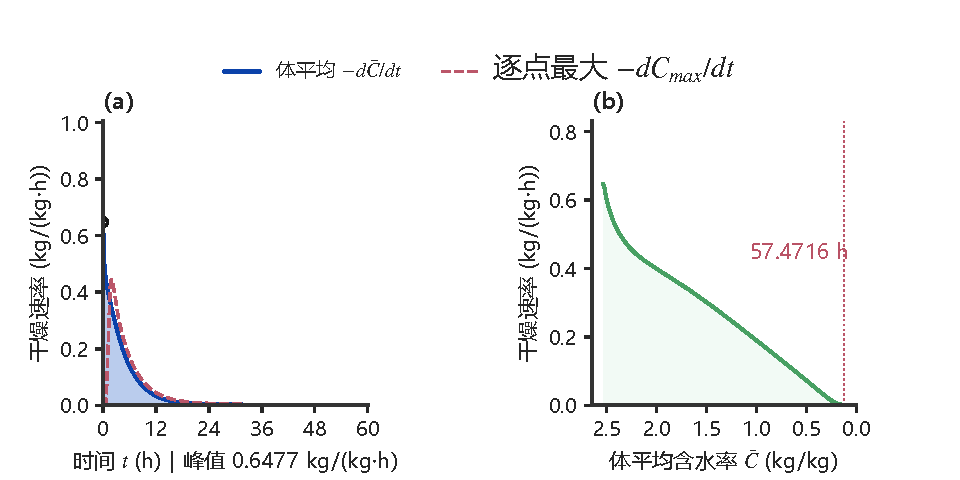
\includegraphics[width=0.9\textwidth,height=0.8\textheight,keepaspectratio]{../figures/fig_q3_rate_curve.pdf}
  \caption{问题三干燥速率的两种读法}
  \label{fig:q3_rate_curve}
\end{figure}

面板 (a) 显示速率峰值 $0.6899$~kg/(kg$\cdot$h) 出现在 $t=0$ 而非某个中间时刻，
此后单调衰减，说明本题不存在升速段。面板 (b) 按 Krischer 的方式把速率对体平均含水率作图，
横轴反向以顺应干燥进程；图中没有出现水平段，即不存在恒速段。
两个面板合起来给出结论：本题自始至终由内部扩散控制，表面蒸发从未成为限制环节。
这与式~\eqref{eq:prop_app3} 中扩散系数强烈依赖含水率的形式一致，
也与前文「限制环节是内部阻力而非供热」的判断相互印证\upcite{Sander1998}。

按题目要求，全过程每隔 $60$~s、距中心每隔 $0.1$~cm 的含水率完整结果保存于结果文件，
覆盖从初始时刻到 $t_{\rm end}$ 的整个过程。
